% !TeX root = ../build/main.tex

\mbi{Change BLAKE2 to Poseidon and leave a footnote.}

In this section, we describe the workflow of Citadel in detail.

\begin{enumerate}

\item (\textbf{user}) $\mathsf{request\_license}()$

	\begin{enumerate}
	
		\item Compute a license stealth address $(\lpk, R_{\lic})$ belonging to the user, using the user's own public key, as follows.
			
			\begin{enumerate}
				\item Sample $r$ uniformly at random from $\F_t$.
				\item Compute a symmetric Diffie--Hellman key $\ksym = rA_{\user}$.
				\item Compute a one-time public key $\lpk = \hb(\ksym)G + B_{\user}$.
				\item Compute $R_{\lic} = rG$.
			\end{enumerate}
		
		\item Compute the license secret key $\lsk = \hb(\ksym) + b_{\user}$ and an additional key $\klic = \hp(\lsk)G$. 
		
		\item Compute the request stealth address $(\rpk, R_{\req})$ using the LP's public key, as follows.
			
			\mbi{Consider using different letter instead of $r$...}
			\begin{enumerate}
				\item Sample $r$ uniformly at random from $\F_t$.
				\item Compute a symmetric Diffie--Hellman key $\kreq = rA_{\LP}$.
				\item Compute a one-time public key $\rpk = \hb(\kreq)G + B_{\LP}$.
				\item Compute $R_{\req} = rG$.
			\end{enumerate}
		
		\item Encrypt data using the key $\kreq$: $\enc = \Enc_{\kreq} ((\lpk, R_{\lic})||\klic; \nonce).$
		
			\mbi{Include how the nonce is computed, if it is a random value as well.}
		
		\item Send the following request to the network: $\req = ((\rpk, R_{\req}), \enc, \nonce).$
		
	\end{enumerate}


\item (\textbf{LP}) $\mathsf{get\_license\_request()}$

	The LP checks continuously the network to detect any incoming license requests addressed to them:
	
	\begin{enumerate}
		\item Compute $\tkreq = a_{\LP}R_{\req}$.
		\item Check if $\rpk \stackrel{?}{=} \hb(\tkreq) G + B_{\LP}$.
	\end{enumerate}
	
	\mbi{Include that if this is the case, the LP should decrypt the encrypted information to retrieve $\lpk, R_{\lic}, \klic$.}
	\mbi{Is this done in $\mathsf{get\_license\_request()}$ or in next step?}

\item (\textbf{LP}) $\mathsf{issue\_license()}$
	
	\begin{enumerate}
		\item Upon receiving a request from a user, define a set of attributes $\attr$ associated to the license, and compute a digital signature as follows:
				$$\lsig = \sign_{\sk_{\SP}}(\lpk, \attr).$$
		\item Encrypt the signature and the attributes using the license key:
			  	$$\enc = \Enc_{\klic} (\lsig || \attr; \nonce).$$
		\item Send the following license to the network:
				$$\lic = ((\lpk, R_{\lic}), \enc, \nonce, \pos).$$
	\end{enumerate}
	
\item (\textbf{user}) $\mathsf{get\_license()}$

	In order to receive the license, the user must scan all incoming transactions the following way:
	
	\begin{enumerate}
		\item Compute $\tklic = \hb(\lsk)G$.
		\item Check if $\lpk \stackrel{?}{=} \hb(\tklic) G + B_{\user}$, 
	\end{enumerate}	
	
	\mbi{Same as before, we should include the step in which the user decyrpts the information associated to the license.}
	
\item (\textbf{user}) $\mathsf{use\_license()}$

	When using the license, open a session with a specific SP by executing a call to the license contract. The following steps are performed:
	
	\mbi{We should mention something about the \textit{license contract} before this step. Maybe in Section 2 where elements are presented? Add a small section about Dusk's blockchain?}
	%or something like: the actions performed by the user are interactions with a wallet software, etc. (add part of Milosz' explanation there - or leave it to implementation details).
	%discuss this with Xavi.
	
	\begin{itemize}
		\item The user issues a transaction that calls the license contract, which includes a ZKP that is computed out of the gadget depicted in Figure \ref{fig:circuit_prove_nft}. Notice that here, the user signs $\mathsf{session\_hash}$ using $\lsk$. Likewise, the user here will need to compute $\lpk' = \lsk G'$.
		\item The network validators will execute the smart contract, which verifies the proof. Upon success, the following session will be added to a shared list of sessions:
		
		$$\Session = \{\mathsf{session\_hash}, \sessionid, \com_0^{hash}, \com_1, \com_2\},$$
		
		where $\mathsf{session\_hash} = \hp(\pk_{\SP} || r_\mathsf{session})$, and $r_\mathsf{session}$ is sampled uniformly at random from $\F_t$.
		
		
	\end{itemize}
	
\item (\textbf{user}) $\mathsf{request\_service()}$

Request the service to the SP, establishing communication using a secure channel, and providing the session cookie that follows.
	
	$$\SessionCookie = \{\pk_{\mathsf{SP}}, r_\mathsf{session}, \sessionid, \pk_{\LP}, \attr, c, \mathsf{s_0}, \mathsf{s_1}, \mathsf{s_2}\}$$

\mbi{Notation-wise: the acronym $\SessionCookie$ can be confused with the common abbreviation for \texttt{smart contract (sc)}, maybe use a different acronym?}
	
\item (\textbf{SSP}) $\mathsf{get\_session()}$

Receive a $\Session$ from the list of sessions, where $\Session.\sessionid = \SessionCookie.\sessionid$.
	
\item (\textbf{SSP}) $\mathsf{grant\_service()}$

Grant or deny the service upon verification of the following steps:
	
	\begin{itemize}
		\item Check whether the values $(\attr, \pk_{\LP}, c)$ included in the $\SessionCookie$ are correct.
		\item Check whether the opening $(\pk_{\SP}, r_\mathsf{session})$ included in the $\SessionCookie$ matches the $\mathsf{session\_hash}$ found in the $\Session$.
		\item Check whether the openings $((\pk_{\LP}, \mathsf{s_0}), (\attr, \mathsf{s_1}), (c, \mathsf{s_2}))$ included in the $\SessionCookie$ match the\\
			  commitments ($\com_0^{hash}, \com_1, \com_2$) found in the $\Session$.
	\end{itemize}

\end{enumerate}
	
%\begin{figure}[h]
%	\centering
%	\setlength{\fboxsep}{5pt}%
%	\setlength{\fboxrule}{0.3pt}%
%	\fbox{
%		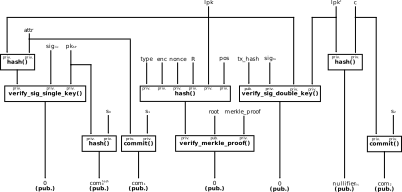
\includegraphics[width=460pt,draft=false]{images/circuit_prove_nft.eps}}
%	\caption{Arithmetic circuit for proving a license's ownership.}
%	\label{fig:circuit_prove_nft}
%\end{figure}

Furthermore, the SP might want to prevent the user from using the license more than once (e.g. this is a single-use license, like entering a concert). This is done through the computation of $\sessionid$. The deployment of this part of the circuit has two different possibilities:
\begin{itemize}
	\item If we set $c = 0$ (or directly remove this input from the circuit), the license can be used only once.
	\item If the SP requests the user to set a custom value for $c$ (e.g. the date of an event), the license can be reused only under certain conditions.
\end{itemize}

